\chapter{DESIGN OF A DECOUPLED SLIDING MODE CONTROL FOR FOUR-LEG DISTRIBUTION STATIC COMPENSATOR}
\label{4.Chap:DSTATCOM}
\section{INTRODUCTION} 
In the previous chapters, the performance characteristics of dual-output converter based UPQC and its control are presented. The control scheme for DOC should incorporate the control of neutral-point voltage (NPV) or common mode voltage (CMV) in addition to the control of inverter currents or voltages. It is also well known that the UPQC is a combination of DSTATCOM and DVR. As an initial step, the control scheme which incorporates the control of NPV is developed for DSTATCOM, later this is applied for shunt terminal of DOC based UPQC in Chapter \ref{6.Chap:DOCUPQC}. 

It is common that three-phase four-wire distribution system experiences unbalance in the load or source, which results in an increased neutral current, thereby resulting in increased power loss and undesirable operation of loads. To control the neutral current or zero sequence and DC currents, the four-leg voltage source converter (FL-VSC) is the best-suited topology as it requires lower DC-link voltage, smaller DC-link capacitor, and simpler control requirement compared to split capacitor three-phase four-wire inverter \cite{5332351,9183965, 8295220}.

For efficient performance of DSTATCOM, an appropriate algorithm comprising the generation of compensator reference currents, and the controller is required. Various theories are discussed in Chapter \ref{2.Chap:DOCIntro} for the generation of compensator reference currents. It is also discussed that designing the complete control algorithm in the natural reference frame ($abc$ frame) makes it insensitive to the signal transformation errors and free from computational burden to some extent. Nonlinear controllers are best choice in the $abc$ frame as their reference tracking capability is unaltered irrespective of the signal frequency. In this chapter, the sliding mode controller is considered due to its robustness against model inaccuracies and lesser computational burden on digital processor as compared to the model predictive controller.  Also among the theories presented in Chapter \ref{2.Chap:DOCIntro}, ISCT is the only choice to design in $abc$ frame. There are other theories in the literature such as least-mean-square (LMS) method \cite{9183965,9516846}, variable forgetting factor recursive least square (VFFRLS) \cite{7084175} and kernel incremental meta-learning (KIM) \cite{6782746} algorithms for generation of compensator reference currents in $abc$ frame. However, ISCT is considered in this chapter due to its less computation requirement.

In the natural reference frame, the current dynamics of a DSTATCOM are coupled through converter pole voltages due to either load neutral-point voltage (NPV) or filter inductance of the converter fourth-leg. This coupling among $a, b, c$ phases leads to cross-coupling in the sliding variable equations with respect to four manipulated input variables, when the conventional sliding surface is chosen. This is why, the controller is generally implemented either in $\alpha\beta$ or $dq$ or $\gamma\theta$ frame \cite{9108551,8616892,8264745}, thereby the coupling effect is avoided. Further, in the conventional SMC and hysteresis current control (HCC) schemes, the currents through the four legs of a DSTATCOM converter are controlled based on corresponding phase current error. However, the four currents in a four-wire system can not be independently controlled variables and hence the role of one of the four controllers is redundant in the conventional control schemes. Considering the coupling issue and the controller redundancy, in this chapter, a new sliding surface is proposed in the natural reference frame itself to get a decoupled feature with respect to the manipulated inputs. It is ensured that the proposed sliding surface is a function of load NPV, thereby the control of NPV is achieved which is useful for the control of DOC based UPQC. 

Finally, the performance of a DSTATCOM with the proposed control scheme under various operating conditions is demonstrated through detailed simulation study and validated with experimental results obtained from a laboratory prototype of the four-leg DSTATCOM.
\vspace*{-1cm}
\section{SYSTEM MODELING AND CONVENTIONAL SLIDING MODE CONTROL}
\noindent The figure provided in Fig.\,\ref{fig4.1} depicts the schematic of a DSTATCOM with a four-leg voltage source converter, which is connected to a three-phase four-wire distribution system. In this section, the mathematical model of a four-leg DSTATCOM in the natural reference frame is reviewed. The objective is to analyze the presence of cross-coupling in the sliding variable equations in relation to the four manipulated input variables.
\begin{figure*}[h]\centering
	\includegraphics[scale=0.7]{figures/Chapter_4/Mine/4leg_DSTATCOM.pdf}
	\caption{Schematic diagram of four-leg voltage source converter based DSTATCOM} 
	\label{fig4.1}
\end{figure*}\vspace*{-1cm} 

\subsection{Modeling of Four-leg DSTATCOM}
To gain a better understanding of the system's dynamic equations given below, Fig.\,\ref{fig4.1} illustrates the extended split capacitor-based DC-link configuration.  
\begin{equation} \label{4.1}
	\begin{aligned}
		v_{jo} & = L_{sh}\frac{di_{shj}}{dt} + v_{gj} + v_{No} + d_{j}  \\
		i_{shf} & =	-\sum_{i=\{a,b,c\}} i_{shi} 	
	\end{aligned}
\end{equation}
Where $j ~ \epsilon ~ \{a,b,c,f\}$, $v_{jo}$ is the pole voltage of four-leg converter, measured disturbance ($v_{gj}$) is grid voltage, controlled variable ($i_{shj}$) and $L_{sh}$ are current and filter inductance of DSTATCOM respectively. Note that $v_{gf}=0$ and unmeasured disturbance ($ d_{j} $) represents the un-modeled dynamics, model mismatch, and variations in model parameters and signal estimations. The load NPV, $v_{No}$ is the voltage between grid neutral `$N$' or load neutral `$N^{\prime}$' to the DC-link midpoint `$o$'. The expression for load NPV is obtained by summing up all pole voltages of \eqref{4.1}. 
\begin{equation} \label{4.2}
	\ v_{No} = \frac{1}{4} \sum_{j} (v_{jo} - v_{gj} - d_{j}) \\
\end{equation}
The pole voltage, $v_{jo}$, always remains within the limits of $\pm0.5 v_{dc}$, where $v_{dc}$ represents the voltage of the DC-link capacitor. Mathematically, this constraint can be expressed as $ v_{jo} = u_{j}\frac{v_{dc}}{2} $, where $u_{j}$ is a manipulated input variable. Specifically, when the top switch of the $j^{th}$ leg ($S_{j}$) is turned ON and its corresponding bottom switch ($\bar{S}_{j}$) is turned OFF, $u_{j} $ is assigned a value of $+1$. Conversely, when the top switch is OFF and the bottom switch is ON, $u_{j} $ is assigned a value of $-1$. With this understanding, \eqref{4.2} can be modified as follows.
\begin{equation} \label{4.3}
	\ v_{No} = \frac{1}{4} \sum_{j}\Big(\frac{v_{dc}}{2} u_{j}  - v_{gj} - d_{j} \Big) \\
\end{equation}

Taking into account the constraint that the four-wire system has only three independent controlled currents and substituting \eqref{4.2} into \eqref{4.1}, the following expression is obtained.
\begin{equation} \label{4.3(1)}
	\begin{aligned}
		%\resizebox{0.42\textwidth}{!}{$\displaystyle
			\begin{bmatrix}
			v_{ao}\\
			v_{bo}\\
			v_{co}
			\end{bmatrix}
			= 
			\begin{bmatrix}
			2  & 1       & 1 \\
			1  & 2       & 1 \\
			1  & 1       & 2
			\end{bmatrix}
			L_{sh}
			\begin{bmatrix}
			\dot{i}_{sha}\\
			\dot{i}_{shb}\\
			\dot{i}_{shc}
			\end{bmatrix}
			+
			\begin{bmatrix}
			v_{ga}\\
			v_{gb}\\
			v_{gc}
			\end{bmatrix}
			+
			\begin{bmatrix}
			d_{a}-d_{f}\\
			d_{b}-d_{f}\\
			d_{c}-d_{f}
			\end{bmatrix}
			+
			v_{fo}
			%$} \\
	\end{aligned}
\end{equation} 
The controller determines the values of the three converter pole voltages based on the dynamics of three independent currents when the value of $v_{fo}$ is known. Typically, $v_{fo}$ is set to zero by switching the fourth leg at a user-defined frequency with a 50\% duty cycle \cite{5224000}. However, in some studies, $v_{fo}$ is deliberately considered as a triplen harmonic signal. This configuration allows for the utilization of space vector modulation using carrier-based pulse-width modulation (PWM), providing additional advantages \cite{1262054}. 
\vspace*{-1cm}\subsection{Conventional SMC}
In the conventional sliding mode control (SMC) or hysteresis current control (HCC), the sliding variable $x_j$ is typically defined as the current error variable, as given below. 
\begin{equation} \label{4.4(1)}
	x_{j}  = i_{shj} - i^{*}_{shj}
\end{equation}
Where $i^{*}_{shj}$ is compensator reference current. Based on the polarity of current error, the conventional control law/input is defined as given below.
\begin{equation} \label{4.7(3)}
	u_{j} = - sgn(x_{j})
\end{equation}
Where $sgn(\cdot)$ is a signum function. If the defined control law satisfies the Lyapunov stability criteria, the system trajectory will ultimately converge to the sliding surface, $x_{j} = 0$ within a finite time.

To ensure global asymptotic stability according to the Lyapunov stability criteria, the Lyapunov function $V(x_{j})$ must satisfy the following properties:
\begin{enumerate}
	\item $V(x_{j}) = 0$ if and only if $x_{j} = 0$
	\item $V(x_{j}) > 0$ if and only if $x_{j} \neq 0$
	\item $\dot{V}(x_{j}) < 0 ~~ \forall ~~ x_{j} \neq 0$  
\end{enumerate}
The time derivative of any signal, say $V(x_{j})$ is denoted as $\dot{V}(x_{j})$ in this paper. Now, the Lyapunov function is selected as below such that the first two properties are satisfied.
\begin{equation} \label{4.6(1)}
	V(x_{j}) = \frac{1}{2} x_{j}^{2}
\end{equation}
To verify the final property, the condition below needs to be satisfied.
\begin{equation} \label{4.7(1)}
	\dot{V}(x_{j}) = x_{j} \dot{x}_{j} < 0
\end{equation}
By substituting the derivative of sliding variable using \eqref{4.3(1)} and \eqref{4.4(1)} into \eqref{4.7(1)}, the following is obtained.
\begin{equation} \label{4.7(2)}
	%\begin{aligned}
		\dot{V}(x_{j}) = x_{j} \frac{1}{4L_{sh}}\bigg\{ \Big[3\Big(u_{j}\frac{v_{dc}}{2} - v_{gj} - d_{j} \Big) - \sum_{\substack{i=\{a,b,c,n\} \\ i \neq j}} \Big(u_{i}\frac{v_{dc}}{2} - v_{gi} -d_{i} \Big) \Big] -4L_{sh}\dot{i}^{*}_{shj}\bigg\} < 0  
	%\end{aligned}
\end{equation}
The condition mentioned above can be satisfied by selecting appropriate manipulated input variables ($u_{a},u_{b},u_{c},u_{f}$). It is evident from \eqref{4.7(2)} that the dynamics of the sliding variable in a specific phase are coupled with the manipulated input variables of other phases. In other words, in order to generate a switching pulse for the converter switches of the phase-$a$ leg, the controller relies on the state of switches in the other three legs. To achieve a decoupled characteristic in terms of the manipulated variables, a new sliding variable is introduced in this chapter.

\section{PROPOSED SLIDING MODE CONTROL SCHEME}
\noindent In this section, the system dynamic equations considering four independent controlled variables and the design of a decoupled sliding mode control are presented.

The equivalent circuit of four-leg DSTATCOM based on \eqref{4.1} is shown in Fig.\,\ref{4.APF_equ}(a). The Thevenin's equivalent impedance observed at the load NPV terminals is shown in Fig.\,\ref{4.APF_equ}(b). The current due to Thevenin's equivalent load NPV, $i_{sh\gamma}$ is given as,  
\begin{equation} \label{4.4}
	i_{sh\gamma} = \frac{4}{L_{sh}} \int v_{No} \, dt.
\end{equation}
\begin{figure}[h!]
	\centering
	\includegraphics[scale=1]{figures/Chapter_4/Mine/APF_equ(a).pdf} \\
	\small (a) 
	\label{4.APF_equ(a)} 
\end{figure}
\begin{figure}[h!]  
	\centering
	\includegraphics[scale=1]{figures/Chapter_4/Mine/APF_equ(d).pdf} \\
	\small (b) 
	\label{4.APF_equ(b)}
	\caption{Four-leg DSTATCOM system: (a) Equivalent circuit, and (b) Thevenin's equivalent impedance seen by load NPV terminals} 
	\label{4.APF_equ}
\end{figure}  
By substituting \eqref{4.4} in \eqref{4.1}, the model equations with four independently controlled variables as given below.
\begin{equation} \label{4.5}
	\begin{aligned}
		%\resizebox{0.45\textwidth}{!}{$\displaystyle
			\begin{bmatrix}
			v_{ao}\\
			v_{bo}\\
			v_{co}\\
			v_{fo}
			\end{bmatrix}
			= 
			\begin{bmatrix}
			1 & 0       & 0       & 0.25 \\
			0       & 1  & 0       & 0.25 \\
			0       & 0       & 1  & 0.25 \\
			-1 & -1 & -1 & 0.25
			\end{bmatrix}
			L_{sh}
			\begin{bmatrix}
			\dot{i}_{sha}\\
			\dot{i}_{shb}\\
			\dot{i}_{shc}\\
			\dot{i}_{sh\gamma}
			\end{bmatrix}
			+
			\begin{bmatrix}
			v_{ga}\\
			v_{gb}\\
			v_{gc}\\
			0
			\end{bmatrix}
			+
			\begin{bmatrix}
			d_{a}\\
			d_{b}\\
			d_{c}\\
			d_{f}
			\end{bmatrix}
		%	$} \\
	\end{aligned}
\end{equation} 
Although the fourth controlled variable, $i_{sh\gamma}$ is a function of load NPV, the load NPV ($v_{No}$) can be estimated using \eqref{4.3} under the assumption that $d_{j} = 0$. However, it is important to consider the mismatch in the estimation of $v_{No}$ and include it in the system dynamic equations presented in \eqref{4.5}. In the conventional DSTATCOM control algorithms, the measurement of grid and DC-link voltages is necessary. Therefore, the proposed algorithm does not require an additional sensor for measuring $v_{No}$.

\vspace*{1cm}
\subsection{SMC Derivation} \label{4.SMC Derivation}
In general, the sliding surface is determined based on the controlled variables. From \eqref{4.5}, it is evident that the converter pole voltage of each phase is influenced by the dynamics of the corresponding phase current and $i_{sh\gamma}$. By selecting a sliding surface for each phase as a combination of the respective phase current and $0.25i_{sh\gamma}$, a decoupled characteristic can be achieved with respect to the manipulated inputs. Therefore, the sliding variable is defined as follows. 
\begin{equation} \label{4.8}
	\sigma_{j} = (i_{shj}+0.25i_{sh\gamma}) - (i^{*}_{shj}+0.25i^{*}_{sh\gamma}) 
\end{equation}
The sliding surface is defined as $\sigma_{j}=0$. The process of generating compensator reference current ($i^{*}_{shj}$) and the reference current due to load NPV ($i^{*}_{sh\gamma}$) is explained later in this section.
To verify the Lyapunov stability condition stated in \eqref{4.7(1)}, the derivative of sliding variable ($\sigma_{j} $) is calculated using \eqref{4.1}, \eqref{4.4}, \eqref{4.5}, and \eqref{4.8}. The expression for the derivative is given below. 
\begin{equation}\label{4.10}
	\begin{aligned}
		\dot{\sigma_{j}} &= \frac{1}{L_{sh}}\Big\{ v_{jo} - \big(L_{sh} \dot{i}^{*}_{shj} + v_{gj} + v^{*}_{No} \big) - d_{j} \Big\} \\
		& = \frac{1}{L_{sh}}\Big\{ u_{j}\frac{v_{dc}}{2} - v^{*}_{jo} - d_{j} \Big\}
	\end{aligned}
\end{equation}
Where $\dot{i}^{*}_{shf} = - \left(\sum_{i=a,b,c}^{}\dot{i}^{*}_{shi}\right) $ and $v^{*}_{No}$ is the load NPV reference. Equation \eqref{4.10} clearly demonstrates that the dynamics of sliding variable associated with a specific phase is entirely decoupled from the manipulated inputs of the other phases. This decoupling property is advantageous for controller design as it allows for the independent evaluation of each component ($a$, $b$, $c$, and $f$) of the four-leg voltage source converter. 

The conventional control law defined in \eqref{4.7(3)} can result in variable and high switching frequency, a phenomenon known as chattering. To mitigate chattering and achieve fixed switching frequency operation, an equivalent control law on the sliding mode can be derived by solving the invariance condition, $\dot{\sigma_{j}} = 0$ \cite{Siew}.
\begin{figure}[b!]   
	\centering
	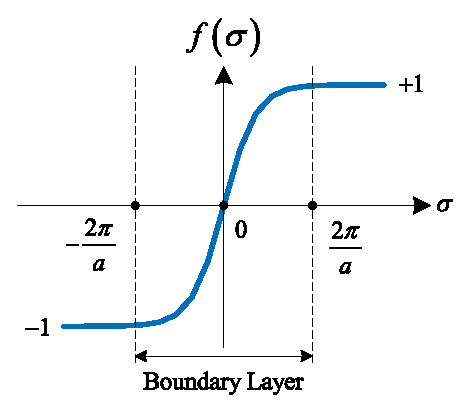
\includegraphics[scale=1]{figures/Chapter_4/Mine/Sigmoid}
	\caption{Hyperbolic tangent control law} 
	\label{4.sigmoid}
\end{figure}
By solving the invariance condition $\dot{\sigma_{j}} = 0$, the resultant equivalent voltage reference signal $\big(v^{eq}_{jo}\big)$ can be obtained as follows.
\begin{equation} \label{4.11}
	v^{eq}_{jo} = v_{jo} = \big(L_{sh} \dot{i}^{*}_{shj} + v_{gj} + v^{*}_{No} \big) + d_{j}
\end{equation} 
In the above equation,  it is not possible to compute $v^{eq}_{jo}$ directly because the instantaneous value of $d_{j}$ is unknown. To address this issue, the un-modeled dynamics ($d_{j}$) are replaced with a control law \big[$-kf(\sigma_{j})$\big], and the modified converter reference voltage ($v^{con}_{jo}$) is computed as given below,  
\begin{equation} \label{4.12}
	v^{con}_{jo} = \big(L_{sh} \dot{i}^{*}_{shj} + v_{gj} + v^{*}_{No} \big) - kf(\sigma_{j}), 
\end{equation}
where $k$ is the control gain and $f(\sigma_{j})$ is generally a signum function. The signum function provides a high gain even when the state trajectory is close to the surface $\sigma_{j} = 0$. This causes the trajectory to move faster and enables it to cross the surface in less time. Consequently, the value of the signum function changes rapidly, resulting in multiple switchings within the designated switching period. To avoid these multiple switchings, the signum function is substituted with a hyperbolic tangent (\textit{tanh}) function as given below. 
\begin{equation} \label{4.13}
	f(\sigma_{j}) = \tanh\Big(\frac{a\sigma_{j}}{2} \Big) ~~ \forall ~\, a > 0
\end{equation} 
In the above equation, the parameter $a$ determines the width of the boundary layer for the \textit{tanh} function, as illustrated in Fig.\,\ref{4.sigmoid}. A lower value of $a$ results in a smoother \textit{tanh} function, eliminating multiple switchings. This leads to reduced switching losses and improved switch lifespan. The proposed SMC computes the four reference voltages using \eqref{4.12} and compares them with a triangular carrier wave of user-defined frequency. This comparison generates the gate pulses for the four-leg DSTATCOM converter switches.  

\vspace*{-0.9cm}
\subsection{Selection of The Proposed SMC Parameters}

Based on Lyapunov stability criteria, the parameters of equivalent control concept of SMC are selected. To verify the stability condition given in \eqref{4.7(1)}, the derivative of sliding variable $\dot{\sigma_{j}}$ is obtained as below by substituting $v_{jo}$ of \eqref{4.10} with $v^{con}_{jo}$ of \eqref{4.12}.
\begin{equation} \label{4.14} 
	\begin{aligned}
		\dot{\sigma_{j}} & = \frac{1}{L_{sh}}\Big\{-kf(\sigma_{j}) - d_{j}\Big\} \\ 
		& = -\frac{k}{L_{sh}}\tanh\Big(\frac{a\sigma_{j}}{2} \Big) - \frac{d_{j}}{L_{sh}}
	\end{aligned}
\end{equation}
Substituting \eqref{4.14} into \eqref{4.7(1)} gives,
\begin{equation} \label{4.15}
	\begin{aligned}
		\dot{V}(\sigma_{j}) & = -\frac{k}{L_{sh}} \sigma_{j} \tanh\Big(\frac{a\sigma_{j}}{2} \Big) - \sigma_{j}\frac{d_{j}}{L_{sh}}  \\
		& \leq \, \frac{\vert \sigma_{j} \vert}{L_{sh}} \Big\{ \vert d_{j}\vert - k sgn(\sigma_{j}) \tanh\Big(\frac{a\sigma_{j}}{2} \Big) \Big\}. 
	\end{aligned}
\end{equation}
For a system trajectory beyond the boundary layer, $sgn(\sigma_{j}) \tanh\Big(\frac{a\sigma_{j}}{2} \Big) = 1$ and as a result, \eqref{4.15} becomes similar to that of the signum function, as given below: 
\begin{equation}
	\dot{V}(\sigma_{j}) \, \leq \, \frac{\vert \sigma_{j} \vert}{L_{sh}} \Big\{ \vert d_{j}\vert - k \Big\}. 
\end{equation}
When the value of $k$ is chosen to be greater than the estimated uncertainties $|d_j|$, the final property of Lyapunov stability criteria, $\dot{V}(\sigma_{j}) < 0$, is satisfied. This ensures global asymptotic stability. However, inside the boundary layer, this stability property fails for the same value of $k$, as $k sgn(\sigma_{j}) \tanh\Big(\frac{a\sigma_{j}}{2} \Big) < \vert d_{j}\vert$. This means that the controller loses its robustness within the boundary layer, and the system dynamics become unpredictable. Consequently, state trajectories always converge to the boundary layer, but they may or may not converge to the surface $\sigma_{j} = 0$. In a pessimistic scenario where state trajectories always diverge within the boundary layer, a steady-state error proportional to the width of the boundary layer arises. It can be inferred that a higher value of $a$ leads to a lower steady-state error. However, increasing the parameter $a$ also increases the number of switchings within the designed switching period, as explained in Section \ref{4.SMC Derivation}. Therefore, the selection of $a$ involves a trade-off between tracking error and multiple switchings.

\vspace*{-0.5cm}
\subsection{Generation of Compensator Reference Quantities and Switching Pulses}
The reference compensator currents are generated using instantaneous symmetrical component theory (ISCT) \cite{4519806} as given below, 
\begin{equation} \label{4.20}
	i^{*}_{shj} = i_{lj} - \frac{v^{+}_{g1j}}{\sum_{k=a,b,c}^{}\left(v^{+}_{g1k}\right)^{2}} \left(P_{lavg} + P_{closs\textunderscore avg}\right), 
\end{equation}
where $P_{lavg}$ and $P_{closs\textunderscore avg}$ are average load power and converter power losses, respectively. The converter power loss is determined by the error in the DC-link voltage, which is regulated using a PI controller. To extract the fundamental positive sequence component of the grid voltages $v^{+}_{g1j}$, the cascaded delayed signal cancellation (CDSC) operator, introduced in \cite{5443553}, is employed. The CDSC operator has been shown to outperform the commonly used second-order generalized integrator (SOGI) \cite{9070288}. 

The reference current $i^{*}_{sh\gamma}$, corresponding to the Thevenin's equivalent load NPV, is determined by integrating $v^{*}_{No}$ based on \eqref{4.4} and it is mathematically expressed as below:
\begin{equation} \label{4.41}
	i^{*}_{sh\gamma} = \frac{4}{L_{sh}} \int v^{*}_{No} \, dt.
\end{equation}
The load NPV reference $v^{*}_{No}$ is a user-defined zero-sequence voltage that depends on the specific application of the converter. In certain cases, such as in a dual-output converter based power quality conditioner, $v^{*}_{No}$ can be a positive DC offset for an upper port or a negative DC offset for a lower port \cite{7018088}. Alternatively, in other applications, $v^{*}_{No}$ can be chosen as triplen harmonics to take advantage of a space vector pulse width modulation (PWM) scheme using a simple carrier-based PWM scheme \cite{1262054}. In this chapter, the proposed control scheme's performance is evaluated by considering both DC offset and triplen harmonics for $v^{*}_{No}$.

The generated reference quantities are utilized to compute the converter reference voltage  $v^{con}_{jo}$ using \eqref{4.12}. These reference voltages are then fed into a sinusoidal pulse width modulator (SPWM) to generate gate pulses for the power switches of the four-leg DSTATCOM. The control block diagram of the proposed sliding mode control (SMC) scheme for the four-leg DSTATCOM is depicted in Fig.\,\ref{fig4.6}.
\begin{figure}[t!]
	\centering
	\includegraphics[scale=1]{figures/Chapter_4/Mine/Control_Diagram.pdf}
	\caption{Block diagram of the proposed SMC control scheme for DSTATCOM} 
	\label{fig4.6}
\end{figure} 

\vspace*{-0.5cm}
\subsection{Design of Filter Inductance}
The design of filter inductance ($L_{sh}$) is same as the conventional approaches as given below.

Consider an equivalent circuit of four-leg DSTATCOM as shown in Fig.\,\ref{4.APF_equ}(a). When the top switch of phase-$a$ leg is turned ON, then the dynamic equation of DSTATCOM is defined as follows:
\begin{equation} \label{4.42}
L_{sh}\frac{\triangle i_{sha}}{T_{on}} = \frac{v_{dc}}{2} - v_{ga} - v_{No},
\end{equation}
where $T_{on}$ is the ON time of top switch, and $\triangle i_{sha}$ is the change in phase-$a$ current of DSTATCOM or DSTATCOM ripple current in phase-$a$. Similarly, when the top switch of phase-$a$ leg is turned OFF, then the dynamic equation of DSTATCOM is defined as follows:
\begin{equation} \label{4.43}
L_{sh}\frac{\triangle i_{sha}}{T_{off}} = \frac{v_{dc}}{2} + v_{ga} + v_{No}.
\end{equation}
The duty ratio ($D^{*}$) of the sinusoidal pulse-width modulation (SPWM) scheme for the known or reference NPV is given as below.
\begin{equation} \label{4.44}
D^{*} = 0.5 + \frac{v_{ga} + v^{*}_{No}}{v_{dc}}
\end{equation}
Using \eqref{4.42}, \eqref{4.43}, and \eqref{4.44}, the switching period ($T_{sw}$) is obtained as below.
\begin{equation} \label{4.45}
\begin{aligned}
T_{sw} &= T_{on} + T_{off} \\
       &= L_{sh}\frac{\triangle i_{sha}}{v_{dc}} \Bigg\{ \frac{1}{0.5 - \frac{v_{ga} + v_{No}}{v_{dc}}} + \frac{1}{0.5 + \frac{v_{ga} +    v_{No}}{v_{dc}}} \Bigg\} \\
       &= L_{sh}\frac{\triangle i_{sha}}{v_{dc}} \bigg\{ \frac{1}{1-D} + \frac{1}{D}\bigg\}
\end{aligned}
\end{equation}
From the above expression, the ripple in filter current ($\triangle i_{sha}$) is obtained as follows:
\begin{equation} \label{4.46}
\triangle i_{sha} = \frac{v_{dc}(1-D)D}{f_{sw}L_{sh}},
\end{equation}
where $f_{sw}$ is the switching frequency. From \eqref{4.46}, it is evident that the ripple current, $\triangle i_{sha}$ is a function of duty ratio ($D$). Thus using maxima and minima concepts, the maximum value of ripple current, $(\triangle i_{sha})_{max}$ is found at $D=0.5$. Substituting $D=0.5$ in \eqref{4.46}, the following is obtained.
\begin{equation} \label{4.47}
L_{sh} = \frac{0.25\, v_{dc}}{f_{sw}(\triangle i_{sha})_{max}}
\end{equation}
This is the minimum value of inductance required for a maximum allowable peak to peak ripple current. The above expression evidences that the higher value of $L_{sh}$ is required for low power loads and lower value for high power loads. 

Now as per IEEE standard 519-2014, the total current demand distortion for a $I_{sc}/I_{L} < 20$ is 5\%. $I_{sc}$ refers to short circuit current and $I_L$ is the nominal load current. Therefore, $(\triangle i_{sha})_{max}$ is considered as $0.05 \times i_{shp}$, where $i_{shp}$ is the peak of rated filter current, i.e., peak of the load current for DSTATCOM study.

\vspace*{-0.5cm}
\section{SIMULATION STUDIES}
The simulation study presented in \cite{8281573} focuses on the hysteresis current control for a four-leg DSTATCOM, utilizing the system parameters specified in Table\,\ref{Table4.2}. For effective validation of the proposed SMC, a simulation study is carried out in this chapter using the same system parameters given in Table\,\ref{Table4.2}. Both the HCC and proposed SMC control schemes are evaluated with a simulation step time of $10\, \si{\micro s}$.
The DC-link voltage controller gains in the proposed system are computed based on a fast-acting DC-link voltage controller described in \cite{5235863}. The controller gains are determined as follows: $k_{p} = 0.0525$ and $k_{i} = 0.026$. These values are chosen to achieve the desired performance of the DC-link voltage control loop in the system. In the process of selecting the SMC parameters, a simulation is initially performed using a signum function to assess the presence of uncertainties in the model. Satisfactory results are obtained with a signum function when the parameter $k$ is set to 15 or higher. The value of $k$ is chosen as the minimum value that yields satisfactory results, which in this case is $k = 15$. Once the value of $k$ is determined, the signum function is replaced with a hyperbolic tangent (\textit{tanh}) function. The parameter $a$ of the \textit{tanh} function is then varied to achieve limited multiple switchings. In the simulation, it is observed that reduced multiple switchings occur when $a = 10$. Therefore, for the proposed SMC in the simulation, the parameters are chosen as $k = 15$ and $a = 10$ to achieve satisfactory performance with limited multiple switchings. 
\begin{table}[] 
	\centering
	\caption{System parameters for simulation study}
	\label{Table4.2}
	\begin{tabular}{>{\small}l>{\small}l}  
		\hline
		\hline
		\textbf{\footnotesize System parameters} & \textbf{\footnotesize Values}\\
		\hline
		\footnotesize Base quantities & \footnotesize$S_{b} = 16\, \si{kVA}, V_{b} = 230 ~\si{V}$ (L-N RMS)  \\
		\footnotesize Filter parameters & \footnotesize $L_{sh} = 22.5 ~\si{mH}$ \\ 
		\footnotesize DC-link voltage & \footnotesize $V_{dc} = 900 ~\si{V}$ \\
		\footnotesize DC-link capacitor & \footnotesize $C_{dc} = 1050 \, \si{\micro F	}$ \\
		\footnotesize Linear load (full load)  &  \footnotesize $Z_{a} = 100+j30\,\si{\Omega}$ \\ & \footnotesize $Z_{b} = 30+j27.5\, \si{\Omega}$ \\  & \footnotesize $Z_{c} = 15+j12.5\, \si{\Omega}$ \\
		\footnotesize Nonlinear load (full load)  &  \footnotesize $3$-$\phi$ diode bridge rectifier with \\ & \footnotesize $R_{nl} = 20  ~\Omega$,\, $L_{nl} = 0.25 ~\si{H}$ \\ 
		\hline
		\hline 
	\end{tabular} 
\end{table} 

In Figs.\,\ref{fig4.82}-\ref{fig4.8}, various waveforms and frequency spectra are presented to validate the performance of the proposed SMC for the four-leg DSTATCOM. The waveforms are expressed in per unit (p.u.) with respect to base values, while the load NPV and sliding variables are shown in their actual units. The base values are considered as $16\,\si{kVA}$ (3-ph) and $230\,\si{V}$ (L-N RMS).
\begin{figure}[h!]  
	%\begin{minipage}{0.5\textwidth}
		\centering
		\includegraphics[scale=0.9]{figures/Chapter_4/Mine/SimRes1_new.pdf} \\
		%\small (a) \vspace*{0.2cm}
		\caption{Simulation results of grid voltages $(v_{gabc})$, and currents of grid, load and DSTATCOM $(i_{gabcN}, i_{labcN}, i_{shabcf})$ in per unit, load NPV reference $(v^{*}_{No})$ in volts, filtered load NPV $(v_{No\_flt})$ in volts and sliding variables $(\sigma_{abcf})$ in amps during grid voltage variations}
		\label{fig4.82}
	%\end{minipage}
	%\begin{minipage}{0.5\textwidth}
\end{figure} 
\begin{figure}[h!] 
		\centering
		\includegraphics[scale=0.9]{figures/Chapter_4/Mine/SimRes2_new.pdf}\\ 
		%\small (b)
	%\end{minipage}
	\caption{Simulation results of grid voltages $(v_{gabc})$, and currents of grid, load and DSTATCOM $(i_{gabcN}, i_{labcN}, i_{shabcf})$ in per unit, load NPV reference $(v^{*}_{No})$ in volts, filtered load NPV $(v_{No\_flt})$ in volts and sliding variables $(\sigma_{abcf})$ in amps during load curtailment} 
	\label{fig4.8}
\end{figure} 

Fig.\,\ref{fig4.82} depicts the transition of grid voltages from a normal condition to a distorted condition at $t=1\,\si{s}$. In this simulation, the reference load NPV $v^{*}_{No}$ is set as a triplen harmonic signal. On the other hand, Fig.\,\ref{fig4.8} shows the case where $v^{*}_{No}$ is set to zero. At $t=1.5\, \si{s}$, load curtailment is introduced. During all the conditions: load curtailment, normal and distorted conditions, the compensated grid currents are resulted as balanced and in-phase with the grid voltages. The grid neutral current becomes zero, indicating that the DSTATCOM has supplied all load components except the fundamental positive sequence component.

The load NPV is a high-frequency pulsed waveform, therefore it is passed through a low pass filter (LPF) with a desired cut-off frequency of 150\,Hz. The filtered load NPVs, $v_{No\_flt}$, shown in Figs.\,\ref{fig4.82}-\ref{fig4.8}, successfully track the reference load NPV signals, whether they are zero or triplen harmonics. This demonstrates the ability of the proposed algorithm to track both compensator reference currents and load NPVs accurately under various system conditions. The sliding variables $\sigma_{abcf}$ are observed to be close to zero for different system conditions, indicating a good reference tracking accuracy of the proposed algorithm.

In Figs.\,\ref{4.SimTHD1}-\ref{fig4.81}, the frequency spectra of the grid current $i_{ga}$ for both HCC and the proposed SMC-based four-leg DSTATCOM are compared. Fig.\,\ref{4.SimTHD1} represents the spectrum during half load condition, while Fig.\,\ref{fig4.81} represents the spectrum during one-fourth load condition. It can be observed that the spectrum of HCC spreads uniformly up to $10\,\si{kHz}$, whereas the spectrum of the proposed SMC spreads dominantly at integral multiples of $10\,\si{kHz}$. This indicates that HCC operates with a variable switching frequency, while the proposed SMC achieves a constant switching frequency operation.
\begin{figure}[h!]  
	%\begin{minipage}{0.5\textwidth}
		\centering
		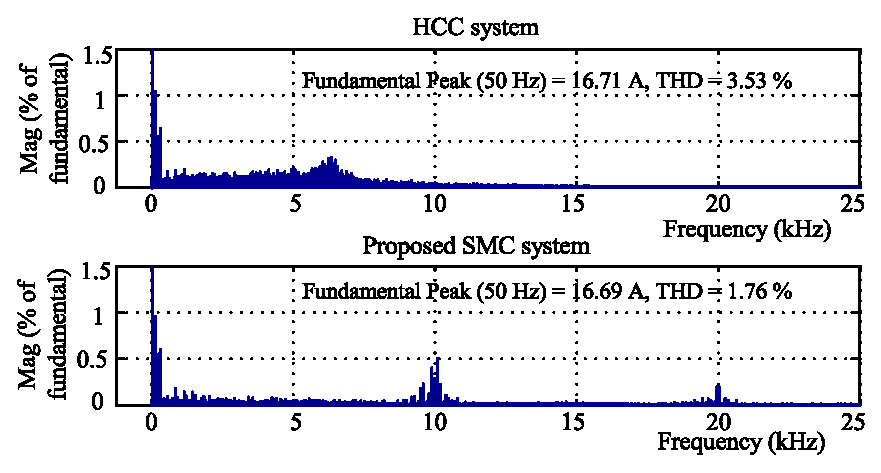
\includegraphics[scale=0.9]{figures/Chapter_4/Mine/SimTHD1.eps}\\ 
		\caption{Simulation results of THD spectrum for phase-$a$ grid current during half load}  
		\label{4.SimTHD1}
	%\end{minipage}
\end{figure}
\begin{figure}[h!]
	%\begin{minipage}{0.5\textwidth}
		\centering
		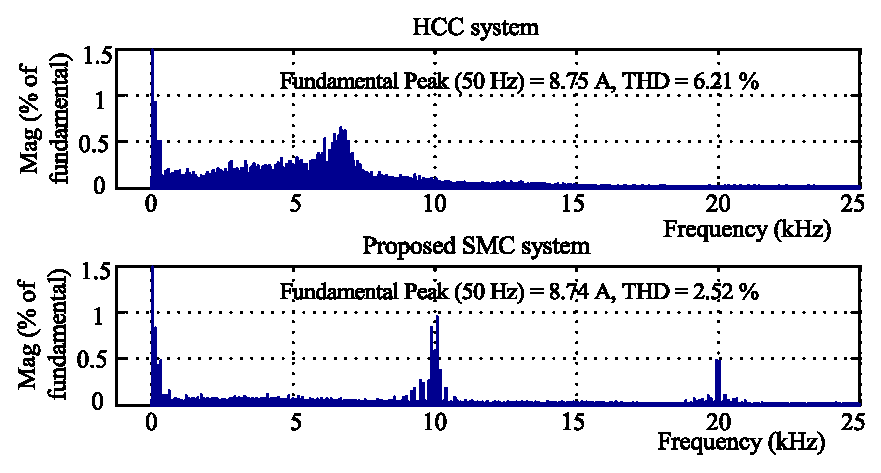
\includegraphics[scale=0.9]{figures/Chapter_4/Mine/SimTHD2.eps}\\
		%\small (b)
		\label{4.SimTHD2}
	%\end{minipage}
	\caption{Simulation results of THD spectrum for phase-$a$ grid current during one fourth load} 
	\label{fig4.81}
\end{figure}
 
\begin{figure}[h!] 
	%\begin{minipage}{0.45\textwidth} 
		\centering
		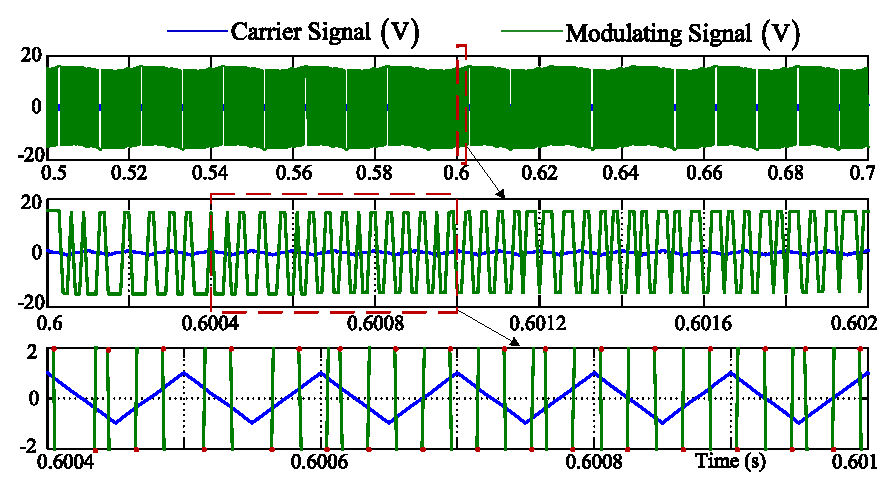
\includegraphics[scale=0.9]{figures/Chapter_4/Mine/Chattering_simulation1.eps}
		\caption{Converter modulating signal of phase-$a$ for \textit{sgn} function}
		\label{4.sign}
	%\end{minipage}
\end{figure}
\begin{figure}[h!] 	
	%\begin{minipage}{0.45\textwidth}
		\centering
		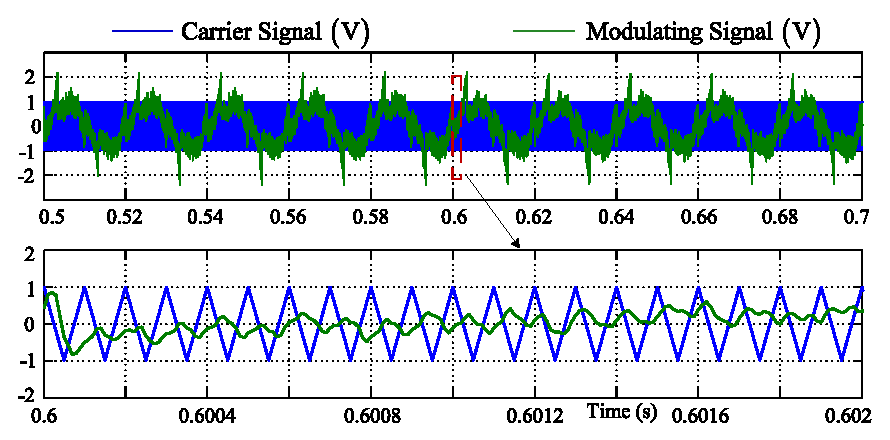
\includegraphics[scale=0.9]{figures/Chapter_4/Mine/Chattering_simulation.eps}
		%\small (b) 
		\label{4.tanh}
%	\end{minipage}
	\caption{Converter modulating signal of phase-$a$ for \textit{tanh} function} 
	\label{4.signtanh}
\end{figure} 

In Figs.\,\ref{4.sign}-\ref{4.signtanh}, a comparison is made between the performance of the conventional signum function and the \textit{tanh} function in terms of the switching pattern for a normal grid condition. Fig.\,\ref{4.sign} shows the modulating signal $(m_{a})$, which is a scaled version of the converter reference voltage of phase-$a$ $(v_{a0}^{con})$ with a carrier wave using the signum function. Fig.\,\ref{4.signtanh} represents the same for the \textit{tanh} function. For both functions, the value of $k$ in \eqref{4.12} is set to $15$, while the value of $a$ for the \textit{tanh} function is set to $10$. It is worth noting that the signum function can be considered as an equivalent of the \textit{tanh} function with $a = \infty$. By comparing the two plots, it is evident that the signum function exhibits multiple crossings between $m_{a}$ and the carrier wave, as observed in the zoomed view in Fig.\,\ref{4.sign}. Conversely, no such multiple crossings are observed in Fig.\,\ref{4.signtanh}. The total harmonic distortions (THDs) of the compensated grid currents $i_{ga},\,i_{gb},\,i_{gc}$ are recorded as 1.62\%, 1.72\%, 1.6\% with the signum function, and 1.76\%, 1.96\%, 1.87\% with the \textit{tanh} function, respectively. These results indicate that the \textit{tanh} function avoids multiple switchings at the expense of slightly higher ripples in the compensated currents compared to the signum function. However, the THDs of the currents remain within the limits specified by IEEE Std. 519. Additionally, it is observed that lower values of $a$ lead to higher THDs, implying higher steady-state errors and fewer multiple switchings. Thus, the selection of $a$ involves a trade-off between steady-state error and multiple switchings. 

To compare the performance of the proposed control scheme with HCC, the THDs of load and grid currents are presented in Fig.\,\ref{4.fig} for various system conditions and parameter variations. In this study, the investigation of controller robustness focuses on two parameters: load power and filter inductance. The THDs of the compensated grid currents shown in Fig.\,\ref{4.fig} under normal grid, distorted grid, full load, half load, and one-fourth load conditions are obtained using a filter inductance of the nominal value, i.e., $L_{sh} =$ 22.5\,mH. The THDs of the compensated grid currents in Fig.\,\ref{4.fig} for the other two cases provide insights into the robustness of the proposed algorithm against variations in the filter inductance. The variations in the filter inductance considered for this study are $L_{sh}\pm 10\,\si{mH}$, where the nominal inductance $L_{sh}$ is 22.5\,mH. The indicated inductance values in Fig.\,\ref{4.fig} are used in the controller for an actual filter inductance of 22.5\,mH. It is observed that the proposed SMC exhibits significantly reduced THDs of grid currents during both normal and distorted grid conditions, indicating its superior performance over HCC and a substantial reduction in chattering. Moreover, both control schemes demonstrate less sensitivity to variations in load power and filter inductance due to their belonging to the variable structure system (VSS) category, which is known for its robustness against unmodeled dynamics. However, the proposed SMC offers greater flexibility with additional control laws, resulting in lower THDs in the compensated grid currents.
\begin{figure}[t]\centering
	\includegraphics[scale=0.5]{figures/Chapter_4/Mine/Bar_Plot.pdf}
	\caption{Performance comparision of HCC and proposed SMC for various system conditions and parameter variations} 
	\label{4.fig}
\end{figure}  

\section{EXPERIMENTAL STUDIES}
A prototype of the four-leg DSTATCOM system, as shown in Fig.\,\ref{fig4.6}, has been developed to compare the performance of the proposed SMC with the HCC system. The experimental study utilizes the system parameters listed in Table\,\ref{Table4.4}. The hardware setup is depicted in Fig.\,\ref{fig4.11}. The four-leg voltage source inverter (VSI) is implemented using IGBT-based SEMIKRON stack. Each leg of the inverter is connected to a similar interfacing inductor. Voltage and current signals are sensed using hall effect transducers and fed to the real-time controller Opal-RT OP4510 (main) and OP4520 (auxiliary) through their analog to digital conversion (ADC) ports. The control algorithm is programmed with a step time of 10 $\mu s$ using the RT-LAB software installed on the host PC. Communication between the real-time controller and the host PC is established via an Ethernet cable, enabling the modification of system parameters such as $k$, $a$, and $v^{*}_{No}$ during the execution of the real-time model.
\begin{table} 
	\centering
	\caption{System parameters for experimental study} 
	\label{Table4.4}
	\begin{tabular}{>{\small}l>{\small}l}  
		\hline
		\hline
		\textbf{\footnotesize System parameters} & \textbf{\footnotesize Values}\\
		\hline
		\footnotesize Base quantities & \footnotesize$S_{b} = 350\, \si{VA}, V_{b} = 50 ~\si{V}$ (L-N RMS)  \\
		\footnotesize Filter parameters & \footnotesize $L_{sh} = 20 \,\si{mH}$ \\ 
		\footnotesize DC-link voltage & \footnotesize $V_{dc} = 200 ~\si{V}$ \\
		\footnotesize DC-link capacitor & \footnotesize $C_{dc} = 2350 \, \si{\micro F	}$ \\
		\footnotesize Linear RL load  &  \footnotesize $Z_{a} = 17+j55.67\,\si{\Omega}$, \\ & \footnotesize $Z_{b} = 50+j58.72\, \si{\Omega}$, \\  & \footnotesize $Z_{c} = 42+j121.2\, \si{\Omega}$. \\
		\footnotesize Resistive load  &  \footnotesize $R_{a} = 48.5\,\si{\Omega}$, \footnotesize $R_{b} = 32\, \si{\Omega}$, \\  & \footnotesize $R_{c} = 54\, \si{\Omega}$ \\
		\footnotesize Nonlinear load  &  \footnotesize $3$-$\phi$ diode bridge rectifier with \\ & \footnotesize $R_{nl} = 92  ~\Omega$,\, $L_{nl} = 85.7 ~\si{mH}$ \\ 
		\footnotesize SMC parameters  &  \footnotesize $a = 20 $,\, $k = 125 $ \\
		\hline
		\hline 
	\end{tabular} 
\end{table}
\begin{figure}[h!]  
	\centering
	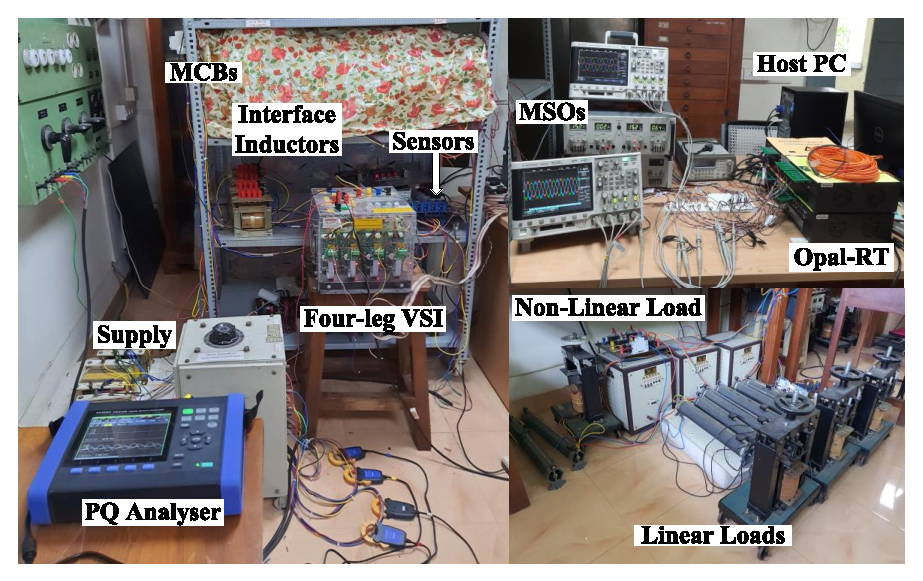
\includegraphics[scale=1]{figures/Chapter_4/Mine/Hardware_Picture_modified.eps}
	\caption{Experimental prototype of the four-leg DSTATCOM}  
	\label{fig4.11}
\end{figure}	

\begin{figure}   
	%\begin{minipage}{0.5\textwidth}
	\centering
	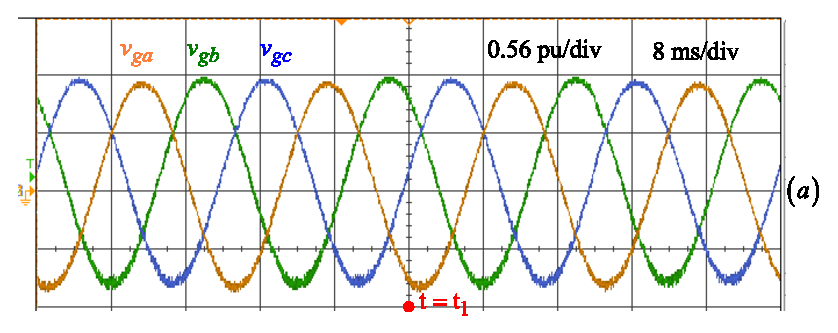
\includegraphics[scale=0.84]{figures/Chapter_4/Mine/GridVoltages.eps}\\ 
	\label{4.gridvolts}
	%\end{minipage}\vspace*{0.2cm}
	%\begin{minipage}{0.5\textwidth}
	\centering
	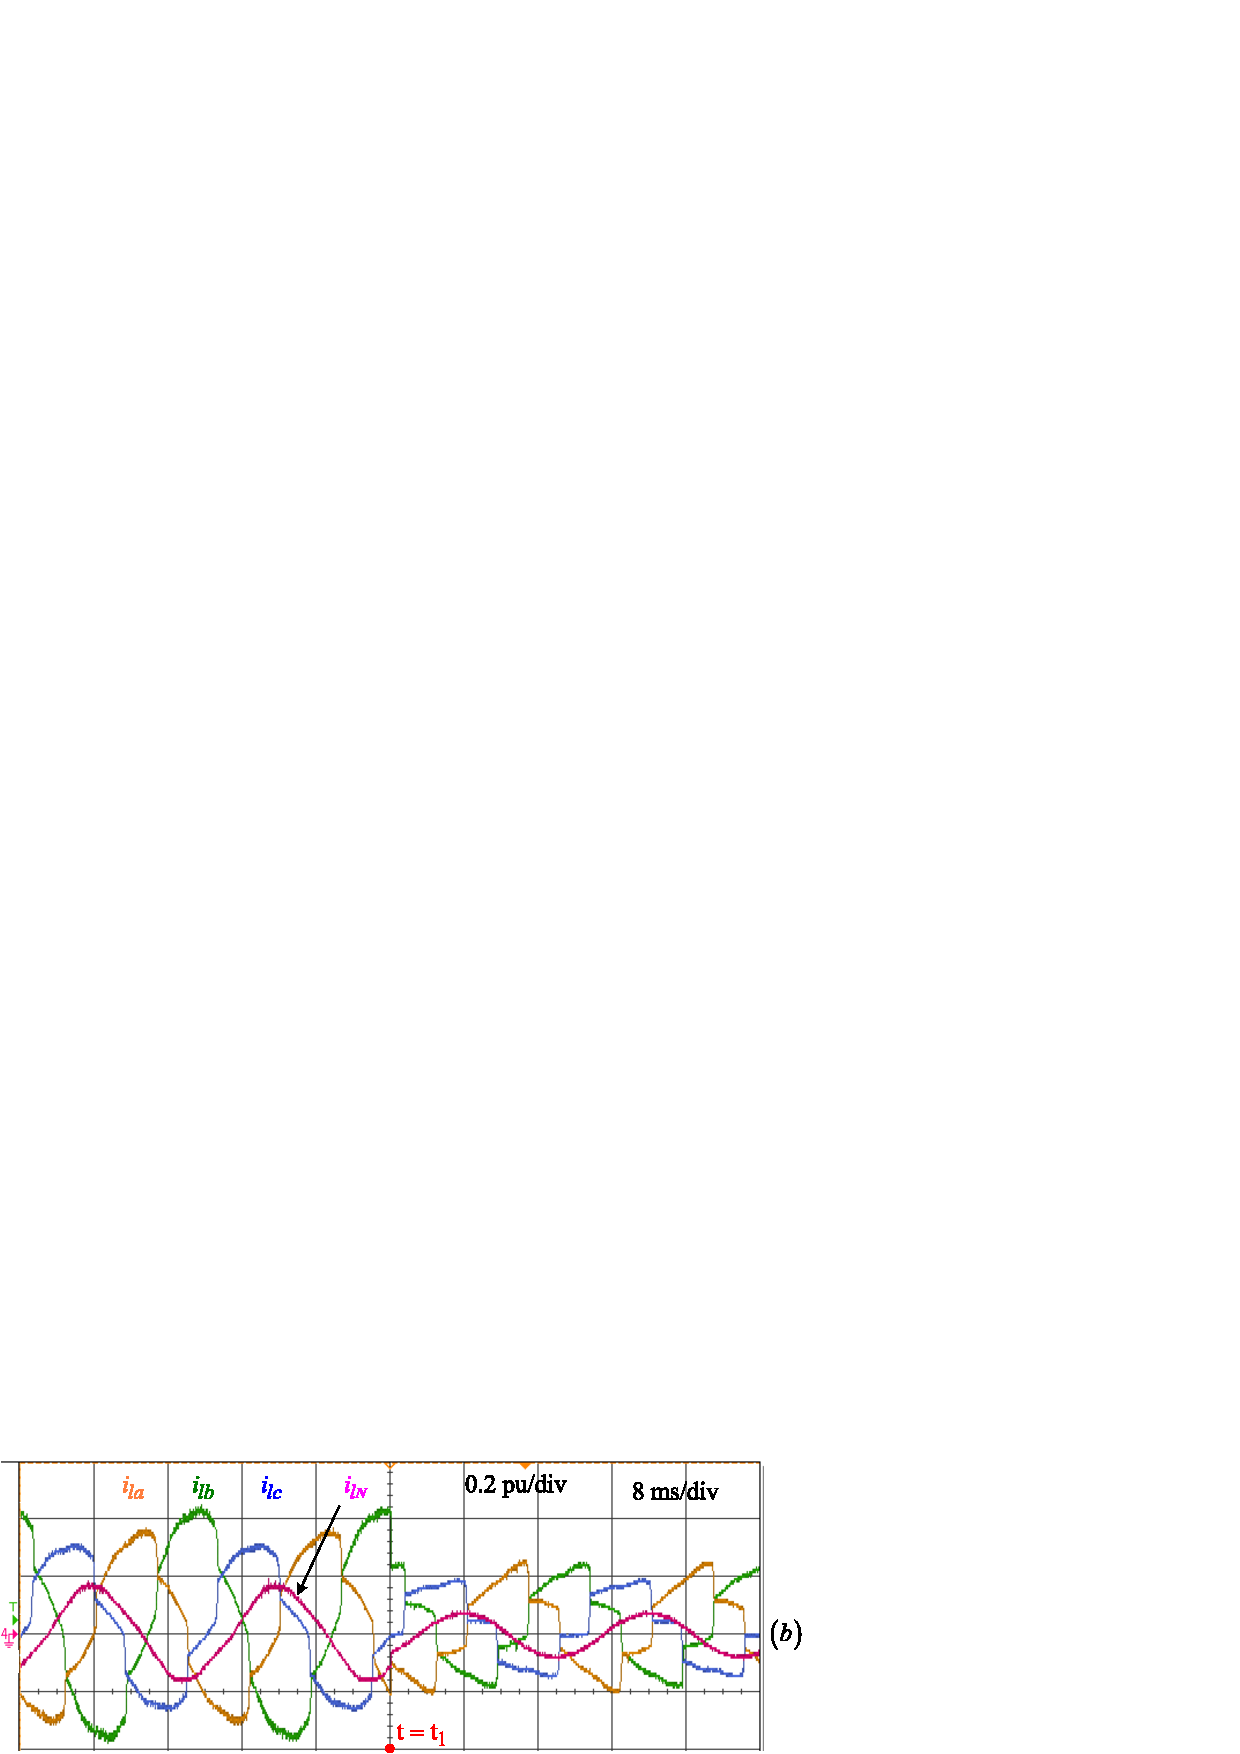
\includegraphics[scale=0.84]{figures/Chapter_4/Mine/LoadCurrents.pdf}\\ 
	\label{4.loadcurrents}
	%\end{minipage}\vspace*{0.2cm}
	%\begin{minipage}{0.5\textwidth}
	\centering
	\includegraphics[scale=0.84]{figures/Chapter_4/Mine/SourceCurrents.pdf}\\ 
	\label{4.sourcecurrents}
	%\end{minipage}\vspace*{0.2cm}
	%\begin{minipage}{0.5\textwidth}
	\centering
	\includegraphics[scale=0.84]{figures/Chapter_4/Mine/FilterCurrents.pdf}\\ 
	\label{4.filtercurrents}
	%\end{minipage}
	%\begin{minipage}{0.5\textwidth}
	\centering
	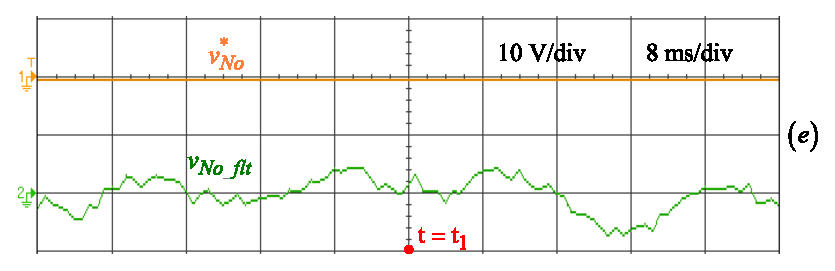
\includegraphics[scale=0.84]{figures/Chapter_4/Mine/LoadNPV.eps}\\ 
	\label{4.LoadNPV}
	%\end{minipage}
	\caption{Experimental results during load curtailment: $(a)$ Grid voltages, $(b)$ Load currents, $(c)$ Grid currents, $(d)$ DSTATCOM currents, and $(e)$ Load neutral-point-voltages}  
	\label{fig4.7}
\end{figure}
\begin{figure}   
	\centering
	\includegraphics[scale=0.9]{figures/Chapter_4/Mine/UPF.pdf}
	\caption{Experimental result: grid voltage and current after compensation} 
	\label{fig4.9}
\end{figure}
In the experimental setup, a three-phase power supply is stepped down to $50\,\si{V}$ ($1\,\si{pu}$) per phase using a three-phase auto transformer, as depicted in Fig.\,\ref{fig4.7}(a). To evaluate the dynamic performance of the four-leg DSTATCOM, a resistive load is suddenly disconnected at time $t=t_{1}$, as shown in Fig.\,\ref{fig4.7}(b). The balanced compensated grid currents in Fig.\,\ref{fig4.7}(c) demonstrate the robustness of the proposed control scheme against load variations. Fig.\,\ref{fig4.7}(d) displays the DSTATCOM currents, where the current through the fourth leg is similar to the load neutral current, resulting in zero current flow through the grid neutral. The reference load NPV ($v^{*}_{No}$) is set to zero, as shown in Fig.\,\ref{fig4.7}(e). The load NPV, which is a high-frequency pulsed waveform, is passed through a low-pass filter (LPF) with a cut-off frequency of 150\,Hz. The filtered load NPV, denoted as $v_{No\_flt}$ in Fig.\,\ref{fig4.7}(e), tracks its reference load NPV of 0\,V. This indicates that the proposed algorithm is capable of tracking both the compensator reference currents and the reference load NPV. Fig.\,\ref{fig4.9} illustrates that the phase difference between the grid voltage and grid current is nearly zero, implying that unity power factor at the grid is achieved by the proposed control scheme.
The percentage THDs of the load currents are 14.1\% (wire $a$), 11.18\% (wire $b$), 14.23\% (wire $c$), and 10.01\% (wire $f$). The frequency spectrum of the compensated grid current, $i_{ga}$, is depicted in Fig.\,\ref{fig4.10} for both the HCC and proposed SMC schemes. It can be observed that the proposed SMC achieves a lower THD compared to the HCC scheme, indicating improved current quality.
\begin{figure}   
	\centering
	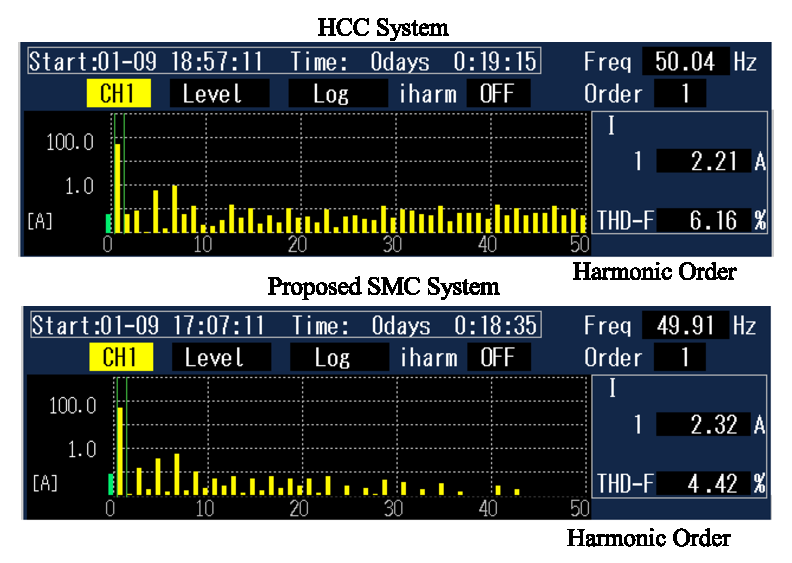
\includegraphics[scale=0.9]{figures/Chapter_4/Mine/THD.eps}
	\caption{Experimental result: frequency spectrum of grid current $i_{ga}$} 
	\label{fig4.10}
\end{figure} 

In Fig.\,\ref{fig4.71}, the performance of the four-leg DSTATCOM at full load condition is demonstrated for a change in the reference load NPV from 50\,V to 0\,V. Fig.\,\ref{fig4.71}(a) shows that the averaged load NPV, $v_{No\_flt}$, tracks the reference load NPV of 50\,V and 0\,V. The load currents, grid currents, and DSTATCOM currents for the variation in reference load NPV are depicted in Figs.\,\ref{fig4.71}(b)-(d), respectively. The balanced grid currents indicate that the compensator with the proposed algorithm has supplied the fundamental reactive and harmonic load currents. Thus, it can be concluded from Fig.\,\ref{fig4.71} that the proposed algorithm is capable of tracking the reference load NPVs in addition to the compensator reference currents.

\begin{figure}    
	%\begin{minipage}{0.5\textwidth}
		\centering
		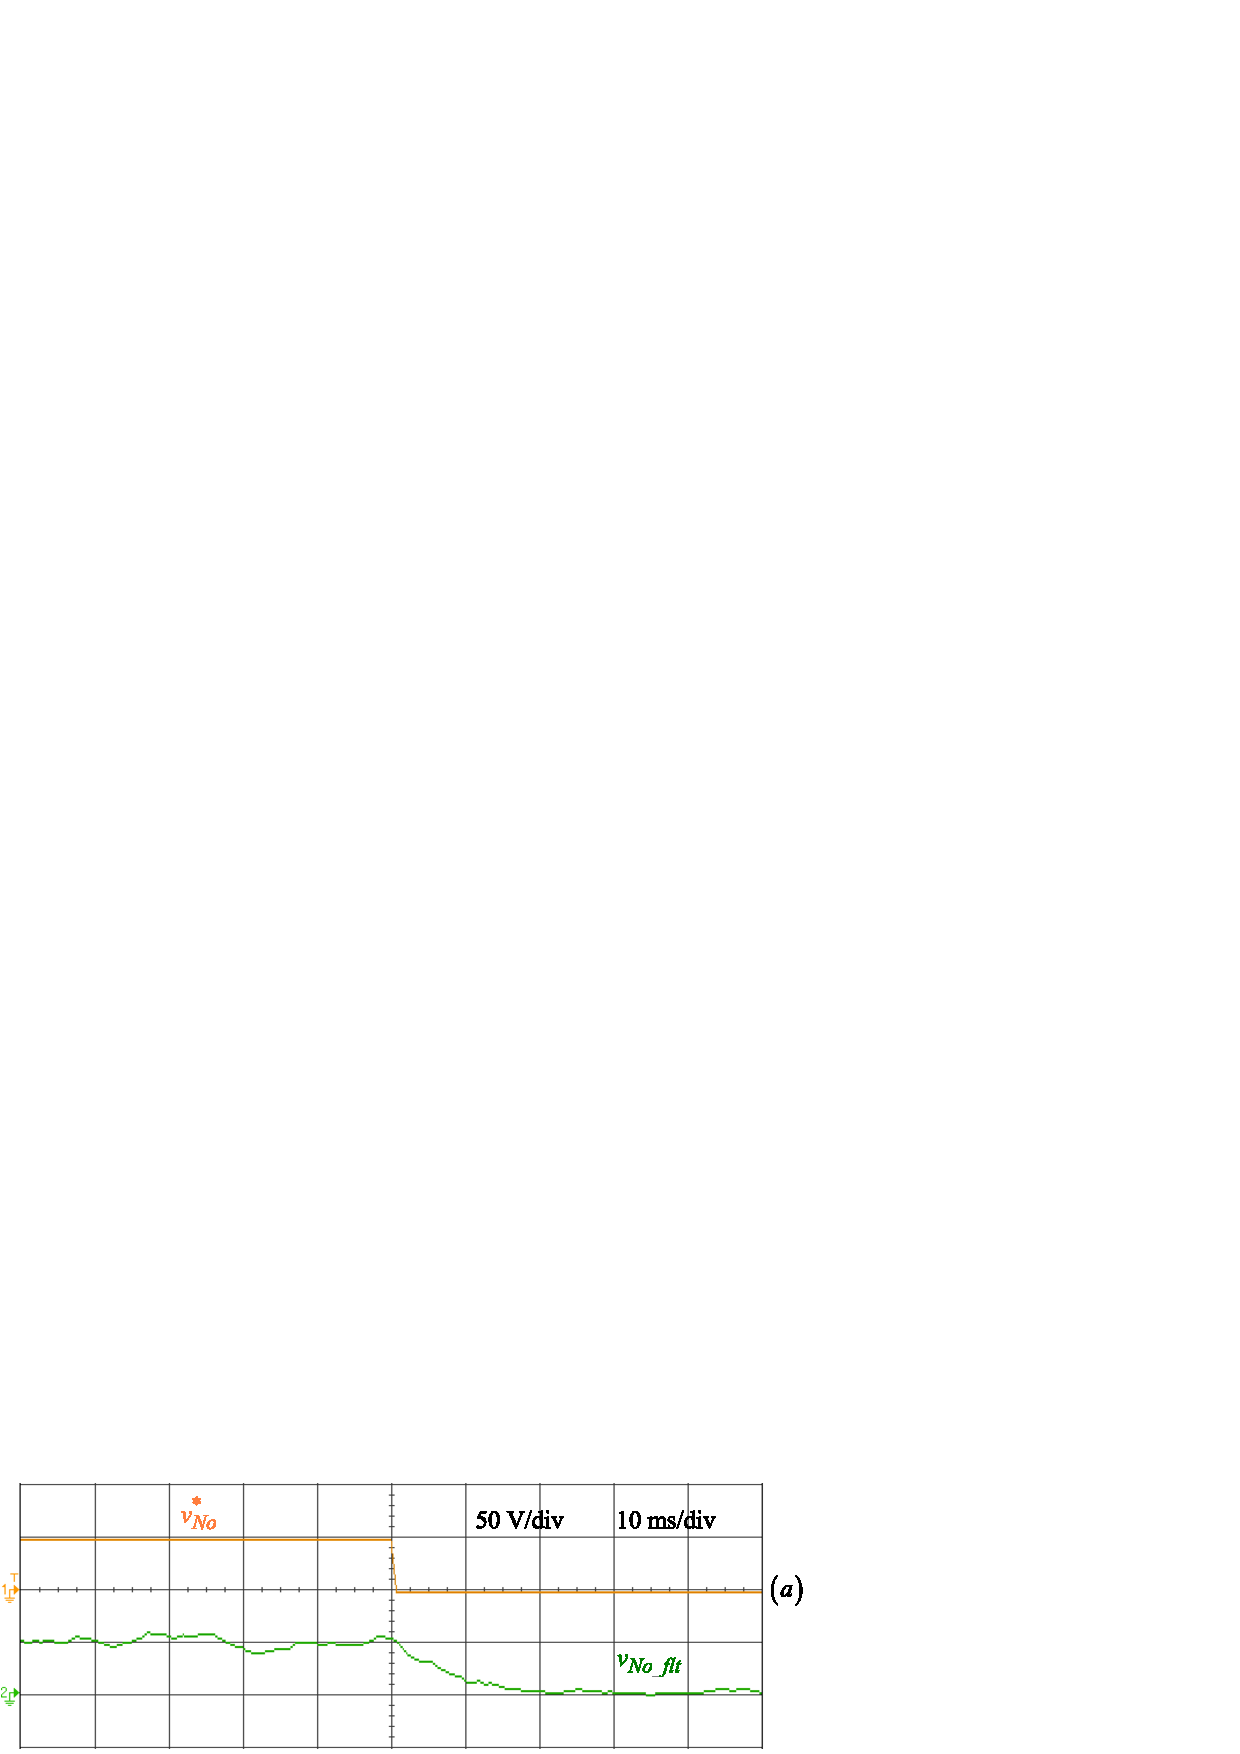
\includegraphics[scale=0.84]{figures/Chapter_4/Mine/LoadNPV1.pdf}\\ 
		\label{4.loadNPV}
	%\end{minipage}\vspace*{0.2cm}
	%\begin{minipage}{0.5\textwidth}
		\centering
		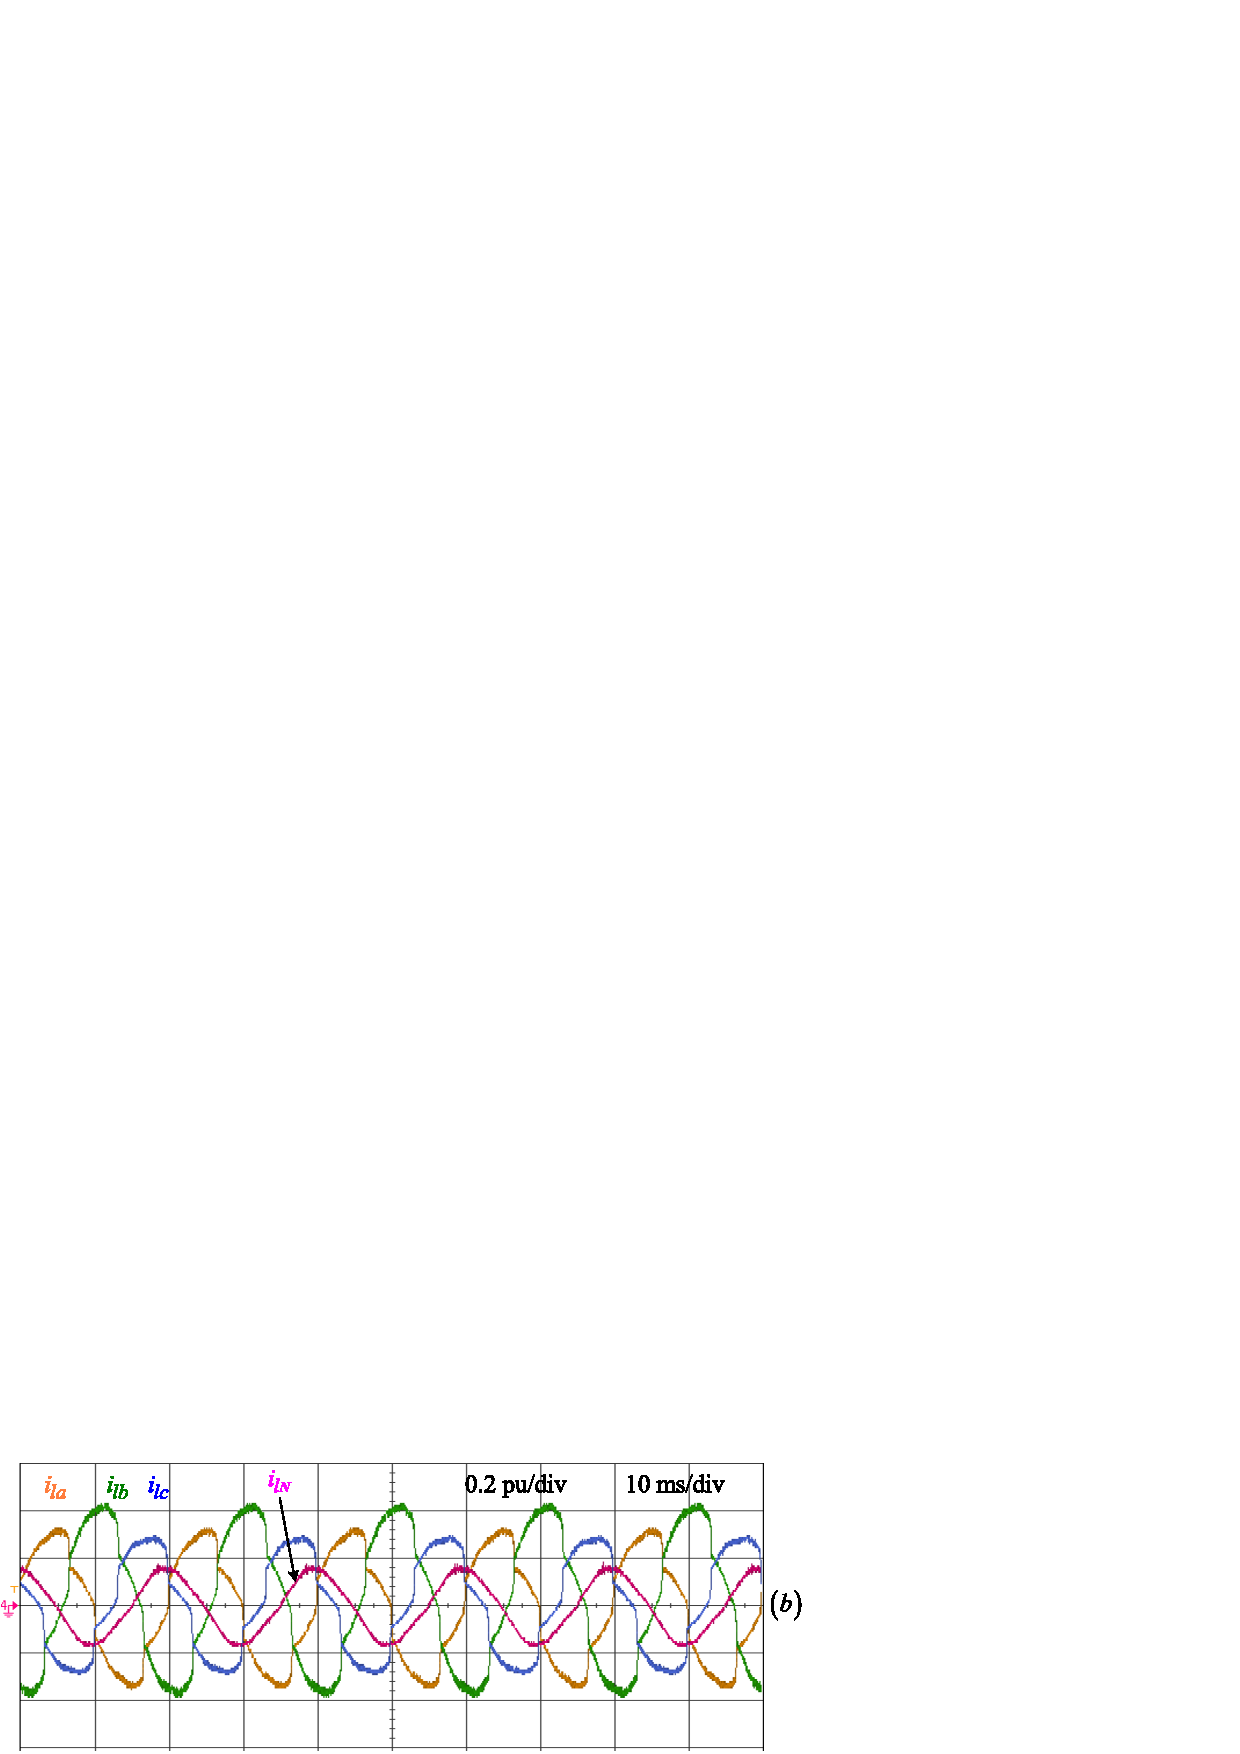
\includegraphics[scale=0.84]{figures/Chapter_4/Mine/LoadCurrents1.pdf}\\ 
		\label{4.loadcurrent}
	%\end{minipage}\vspace*{0.2cm}
	%\begin{minipage}{0.5\textwidth}
		\centering
		\includegraphics[scale=0.84]{figures/Chapter_4/Mine/SourceCurrents1.pdf}\\ 
		\label{4.sourcecurrent}
	%\end{minipage}\vspace*{0.2cm}
	%\begin{minipage}{0.5\textwidth}
		\centering
		\includegraphics[scale=0.84]{figures/Chapter_4/Mine/FilterCurrents1.pdf}\\ 
		\label{4.filtercurrent}
	%\end{minipage}
	\caption{Experimental results during full load condition: $(a)$ Load NPVs, $(b)$ Load currents, $(c)$ Grid currents, and $(d)$ DSTATCOM currents}  \vspace*{-0.5cm}
	\label{fig4.71}
\end{figure}  
\section{STATE-OF-THE-ART AND PROPOSED METHOD COMPARISONS}

Table\,\ref{Table4.3} provides a comparison of the proposed method with state-of-the-art techniques. The method presented in \cite{6880399} has a drawback in that it involves the dq-transformation of various signals and requires multiple PR controllers, each one is responsible for compensating a specific frequency component of the reference currents. However, when the estimation of the grid voltage phase angle is not accurate, the use of dq-transformation introduces errors and inaccuracies in reference tracking. To overcome the limitations of linear controllers, researchers have explored non-linear controllers in the literature. These non-linear controllers aim to achieve robust performance across a wide range of operating conditions.

In the natural reference frame, the current dynamics of a three-wire three-leg or four-leg converter-based DSTATCOM are interconnected through the converter pole voltages, which is a result of the load's neutral-point voltage (NPV). In order to achieve a decoupled characteristic, signals are transformed into a new $\gamma\theta$-frame as described in \cite{8264745}. However, this transformation is susceptible to transformation errors. In contrast, the coupling mentioned above is absent in \cite{8998568} due to the implementation of a split-capacitor based three-leg converter topology. However, this converter topology has certain limitations compared to the four-leg converter topology mentioned in \cite{5332351}. Additionally, the absence of load NPV in the split-capacitor based three-leg converter topology makes it unsuitable for dual-output converter based power quality conditioners.

In the study conducted in \cite{8281573}, one of the four controllers designed is redundant because a four-wire system only has three independent currents. Moreover, the control of load NPV is crucial for dual-output converter based power quality conditioners, as the absence of such control can lead the converter to enter an invalid switching state, resulting in undesired performance. Therefore, the proposed method incorporates load NPV control, whereas it is not incorporated in \cite{6880399,8264745,8281573}, and \cite{8998568}. The control scheme presented in this chapter can be utilized for the control of dual-output converter based power quality conditioners. 

\begin{landscape}
	\begin{table*}[ht] 
		\centering
		\setlength\extrarowheight{2pt}
		\caption{A comparison between the proposed method and the existing techniques} 
		\label{Table4.3}
		\begin{tabular}{>{\small }l>{\small }l>{\small }l>{\small }l>{\small }l>{\small }l}  
			\hline
			\hline
			\textbf{Comparison category} & \textbf{ \cite{6880399}} & \textbf{ \cite{8264745}} & \textbf{\cite{8281573}} & \textbf{\cite{8998568}}  & \textbf{ Proposed method} \\
			\hline
			Converter & Three-wire & Three-wire & Four-wire & Four-wire & Four-wire \\
			topology & three-leg & three-leg & four-leg & three-leg & four-leg \\
			& converter & converter & converter & converter & converter \\
			\hline
			Generation of &SRF & Based on DC-link & ISC & IRP & ISC  \\ 
			compensator reference currents & theory & voltage control & theory & theory & theory \\
			\hline
			Control strategy & Linear PR & SMC & HCC & Second Order SMC & SMC \\
			\hline
			Controller implementation in & $dq$-frame & $\gamma\theta$-frame & Natural frame & Natural frame & Natural frame \\
			\hline
			Constant switching frequency operation  &  Yes & Yes & No & Yes & Yes \\
			\hline
			Ability of load balancing  &  Yes & Yes & Yes & Yes & Yes \\  \hline
			Ability of load NPV control  &  No & No & No & No & Yes \\  
			\hline
			\hline 
		\end{tabular}  
	\end{table*}
\end{landscape}

\section{SUMMARY}
This chapter presents the design of a decoupled sliding mode control scheme for the control of a four-leg DSTATCOM in the natural reference frame. In conventional control schemes, the dynamics of sliding variables are coupled through the manipulated input variables. However, in the proposed scheme, this coupling is eliminated by introducing a new sliding surface function. The redundant current controller found in conventional schemes is utilized in the proposed scheme to control the fourth independent variable, which is the current due to Thevenin's equivalent load NPV. The design of the proposed scheme, which includes load NPV control, is also applicable to the control of dual-output converter based power quality conditioners.

By employing the proposed control scheme, accurate control of load NPV is achieved under various system conditions without compromising the common functionalities of a DSTATCOM. The effectiveness of the proposed scheme is validated through detailed simulations and experimental studies conducted on a four-leg DSTATCOM system. The results of these studies indicate that the proposed control scheme offers the following advantages: (a) robust performance against variations in filter inductances and load powers; (b) operation at a constant switching frequency; and (c) reduced total harmonic distortions (THDs) in the compensated grid currents.